\documentclass[a4paper,14pt]{extarticle}

\usepackage[a4paper,margin=2.5cm]{geometry}
\usepackage{iftex}
\ifPDFTeX
  \usepackage[T2A]{fontenc}
  \usepackage[utf8]{inputenc}
  \usepackage[russian]{babel}
  \usepackage{tempora}
\else
  \usepackage[russian]{babel}
  \usepackage{fontspec}
  \setmainfont{Times New Roman}
\fi

\usepackage{amsmath}
\usepackage{amssymb}
\usepackage{graphicx}
\usepackage{float}
\usepackage{booktabs}
\usepackage{setspace}
\usepackage{xcolor}
\usepackage{listings}
\usepackage{fancyvrb}
\usepackage{subcaption}
\usepackage{caption}
\usepackage[unicode, colorlinks=true, linkcolor=blue, urlcolor=magenta]{hyperref}
\usepackage{listingsutf8}

\onehalfspacing

\definecolor{codegreen}{rgb}{0,0.6,0}
\definecolor{codegray}{rgb}{0.5,0.5,0.5}
\definecolor{codepurple}{rgb}{0.58,0,0.82}
\definecolor{backcolour}{rgb}{0.95,0.95,0.92}

\lstset{
    language=Python,
    backgroundcolor=\color{backcolour},
    commentstyle=\color{codegreen},
    keywordstyle=\color{blue},
    numberstyle=\tiny\color{codegray},
    stringstyle=\color{codepurple},
    basicstyle=\ttfamily\small,
    breakatwhitespace=false,
    breaklines=true,
    captionpos=b,
    keepspaces=true,
    numbers=left,
    numbersep=5pt,
    showspaces=false,
    showstringspaces=false,
    showtabs=false,
    tabsize=2,
    frame=single,
    inputencoding=utf8,
    extendedchars=true,
    texcl=true,
    literate={а}{{\cyra}}1 {б}{{\cyrb}}1 {в}{{\cyrv}}1 {г}{{\cyrg}}1 {д}{{\cyrd}}1 {е}{{\cyre}}1 {ё}{{\"e}}1 {ж}{{\cyrzh}}1 {з}{{\cyrz}}1 {и}{{\cyri}}1 {й}{{\cyrishrt}}1 {к}{{\cyrk}}1 {л}{{\cyrl}}1 {м}{{\cyrm}}1 {н}{{\cyrn}}1 {о}{{\cyro}}1 {п}{{\cyrp}}1 {р}{{\cyrr}}1 {с}{{\cyrs}}1 {т}{{\cyrt}}1 {у}{{\cyru}}1 {ф}{{\cyrf}}1 {х}{{\cyrh}}1 {ц}{{\cyrc}}1 {ч}{{\cyrch}}1 {ш}{{\cyrsh}}1 {щ}{{\cyrshch}}1 {ъ}{{\cyrhrdsn}}1 {ы}{{\cyry}}1 {ь}{{\cyrsftsn}}1 {э}{{\cyrerev}}1 {ю}{{\cyryu}}1 {я}{{\cyrya}}1 {А}{{\CYRA}}1 {Б}{{\CYRB}}1 {В}{{\CYRV}}1 {Г}{{\CYRG}}1 {Д}{{\CYRD}}1 {Е}{{\CYRE}}1 {Ё}{{\"E}}1 {Ж}{{\CYRZH}}1 {З}{{\CYRZ}}1 {И}{{\CYRI}}1 {Й}{{\CYRISHRT}}1 {К}{{\CYRK}}1 {Л}{{\CYRL}}1 {М}{{\CYRM}}1 {Н}{{\CYRN}}1 {О}{{\CYRO}}1 {П}{{\CYRP}}1 {Р}{{\CYRR}}1 {С}{{\CYRS}}1 {Т}{{\CYRT}}1 {У}{{\CYRU}}1 {Ф}{{\CYRF}}1 {Х}{{\CYRH}}1 {Ц}{{\CYRC}}1 {Ч}{{\CYRCH}}1 {Ш}{{\CYRSH}}1 {Щ}{{\CYRSHCH}}1 {Ъ}{{\CYRHRDSN}}1 {Ы}{{\CYRY}}1 {Ь}{{\CYRSFTSN}}1 {Э}{{\CYREREV}}1 {Ю}{{\CYRYU}}1 {Я}{{\CYRYA}}1
}

\begin{document}

\begin{titlepage}
    \centering

    \IfFileExists{fefu.jpg}{
        
\includegraphics[scale=0.15]{fefu.jpg}\\[0.4cm]
    }{
        \vspace*{1.8cm}
    }

    МИНИСТЕРСТВО НАУКИ И ВЫСШЕГО ОБРАЗОВАНИЯ\\
    РОССИЙСКОЙ ФЕДЕРАЦИИ\\
    Федеральное государственное автономное образовательное учреждение высшего образования\\
    \textbf{«Дальневосточный федеральный университет»}\\
    \textbf{(ДВФУ)}\\[0.3cm]
    \rule{\linewidth}{0.7mm}\\[0.3cm]

    \textbf{ИНСТИТУТ МАТЕМАТИКИ И КОМПЬЮТЕРНЫХ ТЕХНОЛОГИЙ}\\[0.3cm]
    \textbf{Кафедра математического и компьютерного моделирования}\\[0.9cm]

    Избосарова Жасмина Олимжоновна\\
    \textbf{ЛАБОРАТОРНАЯ РАБОТА №3: ЭМПИРИЧЕСКАЯ ФУНКЦИЯ РАСПРЕДЕЛЕНИЯ}\\[0.3cm]

    Направление подготовки 02.03.01 СЦТ «Сквозные цифровые технологии»,\\
    образовательная программа «Математика и компьютерные науки»,\\
    очная форма обучения\\[1cm]

    \raggedleft
    \textbf{Студент группы Б9123-02.03.01сцт2}\\
    \rule{4.5cm}{0.3mm} Ж.\,О.~Избосарова\\[1cm]

    \textbf{Руководитель проекта}\\
    \rule{4.2cm}{0.3mm} К.\,А.~Ганжа

    \vfill
    \centering
    Владивосток\\
    2026
\end{titlepage}

\section{ Краткое математическое описание методов и синтаксис в Python}

В работе рассматриваются те же 8 выборок, что и в лабораторной работе №1: по две выборки объёмов \(100\) и \(1000\) из распределений
\[
U(2,7), \qquad B(0.27), \qquad Bin(12,0.35), \qquad N(4.5, 1.8^2).
\]

Для выборки \(X_1,\dots,X_n\) эмпирическая функция распределения определяется формулой
\[
F_n(x)=\frac{1}{n}\sum_{i=1}^{n} I(X_i \le x),
\]
где \(I(X_i \le x)\) --- индикатор того, что наблюдение не превосходит точку \(x\).

Доверительный интервал \(L(x), U(x)\) для \(F(x)\) с уровнем доверия \(1-\alpha\) в нашем случае имеет вид:
\[
\mathbb{P}\bigl(L(x)\le F(x)\le U(x)\bigr)\ge 1-\alpha.
\]

Где:
\[
L(x)=\max\bigl(\hat{F}_n(x)-\varepsilon_n;\,0\bigr),
\]
\[
U(x)=\min\bigl(\hat{F}_n(x)+\varepsilon_n;\,1\bigr),
\]
\[
\varepsilon_n=\sqrt{\frac{1}{2n}\ln\left(\frac{2}{\alpha}\right)}.
\]

В работе используется 95\%-й доверительный интервал, то есть
\[
\alpha=0.05.
\]

В программе нижняя и верхняя границы дополнительно ограничиваются интервалом \([0,1]\), так как функция распределения не может принимать значения вне этого отрезка.

Во всех экспериментах фиксируется
\begin{lstlisting}
random_state = 16
\end{lstlisting}

Генерация выборок выполняется так же, как и в ЛР №1.

Равномерное распределение: \(X \sim U(2,7)\).\\
Код:
\begin{lstlisting}
st.uniform.rvs(loc=2, scale=5, size=100, random_state=16)
st.uniform.rvs(loc=2, scale=5, size=1000, random_state=16)
\end{lstlisting}

Распределение Бернулли: \(X \sim B(0.27)\).\\
Код:
\begin{lstlisting}
st.bernoulli.rvs(p=0.27, size=100, random_state=16)
st.bernoulli.rvs(p=0.27, size=1000, random_state=16)
\end{lstlisting}

Биномиальное распределение: \(X \sim Bin(12,0.35)\).\\
Код:
\begin{lstlisting}
st.binom.rvs(n=12, p=0.35, size=100, random_state=16)
st.binom.rvs(n=12, p=0.35, size=1000, random_state=16)
\end{lstlisting}

Нормальное распределение: \(X \sim N(4.5, 1.8^2)\).\\
Код:
\begin{lstlisting}
st.norm.rvs(loc=4.5, scale=1.8, size=100, random_state=16)
st.norm.rvs(loc=4.5, scale=1.8, size=1000, random_state=16)
\end{lstlisting}

Собственная функция вычисления ЭФР и доверительного интервала имеет вид:
\begin{lstlisting}
def empirical_cdf(sample, x, alpha=0.05):
    sample = np.sort(np.asarray(sample))
    n = sample.size
    x_array = np.atleast_1d(x)

    fn = np.searchsorted(sample, x_array, side="right") / n
    epsilon = np.sqrt(np.log(2 / alpha) / (2 * n))
    lower = np.clip(fn - epsilon, 0.0, 1.0)
    upper = np.clip(fn + epsilon, 0.0, 1.0)

    if np.ndim(x) == 0:
        return float(fn[0]), float(lower[0]), float(upper[0])
    return fn, lower, upper
\end{lstlisting}

Для сравнения используется встроенная функция из \texttt{SciPy}:\\
Код:
\begin{lstlisting}
ecdf_result = st.ecdf(sample)
ecdf_values = ecdf_result.cdf.evaluate(x_grid)
ci = ecdf_result.cdf.confidence_interval(confidence_level=0.95)
low = ci.low.evaluate(x_grid)
high = ci.high.evaluate(x_grid)
\end{lstlisting}

Для непрерывных распределений графики строятся на плотной равномерной сетке по \(x\), а для дискретных --- по целочисленным значениям из области возможных исходов.

\section{ Результаты}

\subsection{ Таблица результатов}

В таблице приведены значения ЭФР в точке медианы каждой выборки, а также нижняя и верхняя границы 95\%-го доверительного интервала.

\begin{table}[h!]
\centering
\caption{Значения ЭФР в точке медианы выборки и 95\%-й доверительный интервал}
\small
\begin{tabular}{lccccc}
\toprule
Выборка & $x$ & $F_n(x)$ & Нижняя граница & Верхняя граница \\
\midrule
uniform\_100 & 4.6254 & 0.5000 & 0.3642 & 0.6358 \\
uniform\_1000 & 4.4807 & 0.5000 & 0.4571 & 0.5429 \\
bernoulli\_100 & 0.0000 & 0.7500 & 0.6142 & 0.8858 \\
bernoulli\_1000 & 0.0000 & 0.7500 & 0.7071 & 0.7929 \\
binom\_100 & 4.0000 & 0.5800 & 0.4442 & 0.7158 \\
binom\_1000 & 4.0000 & 0.5950 & 0.5521 & 0.6379 \\
norm\_100 & 4.6516 & 0.5000 & 0.3642 & 0.6358 \\
norm\_1000 & 4.4144 & 0.5000 & 0.4571 & 0.5429 \\
\bottomrule
\end{tabular}
\end{table}


По таблице видно, что при увеличении объёма выборки доверительный интервал становится уже, а значение ЭФР стабилизируется.

\subsection{ Графики }

На графиках:
\begin{itemize}
\item красная линия --- истинная функция распределения;
\item синяя ступенчатая линия --- эмпирическая функция распределения;
\item зелёные пунктирные линии --- нижняя и верхняя границы 95\%-го доверительного интервала.
\end{itemize}

На первом рисунке приведены результаты для собственной реализации ЭФР и доверительного интервала, построенного по приведённой выше формуле.

\begin{figure}[H]
    \centering
    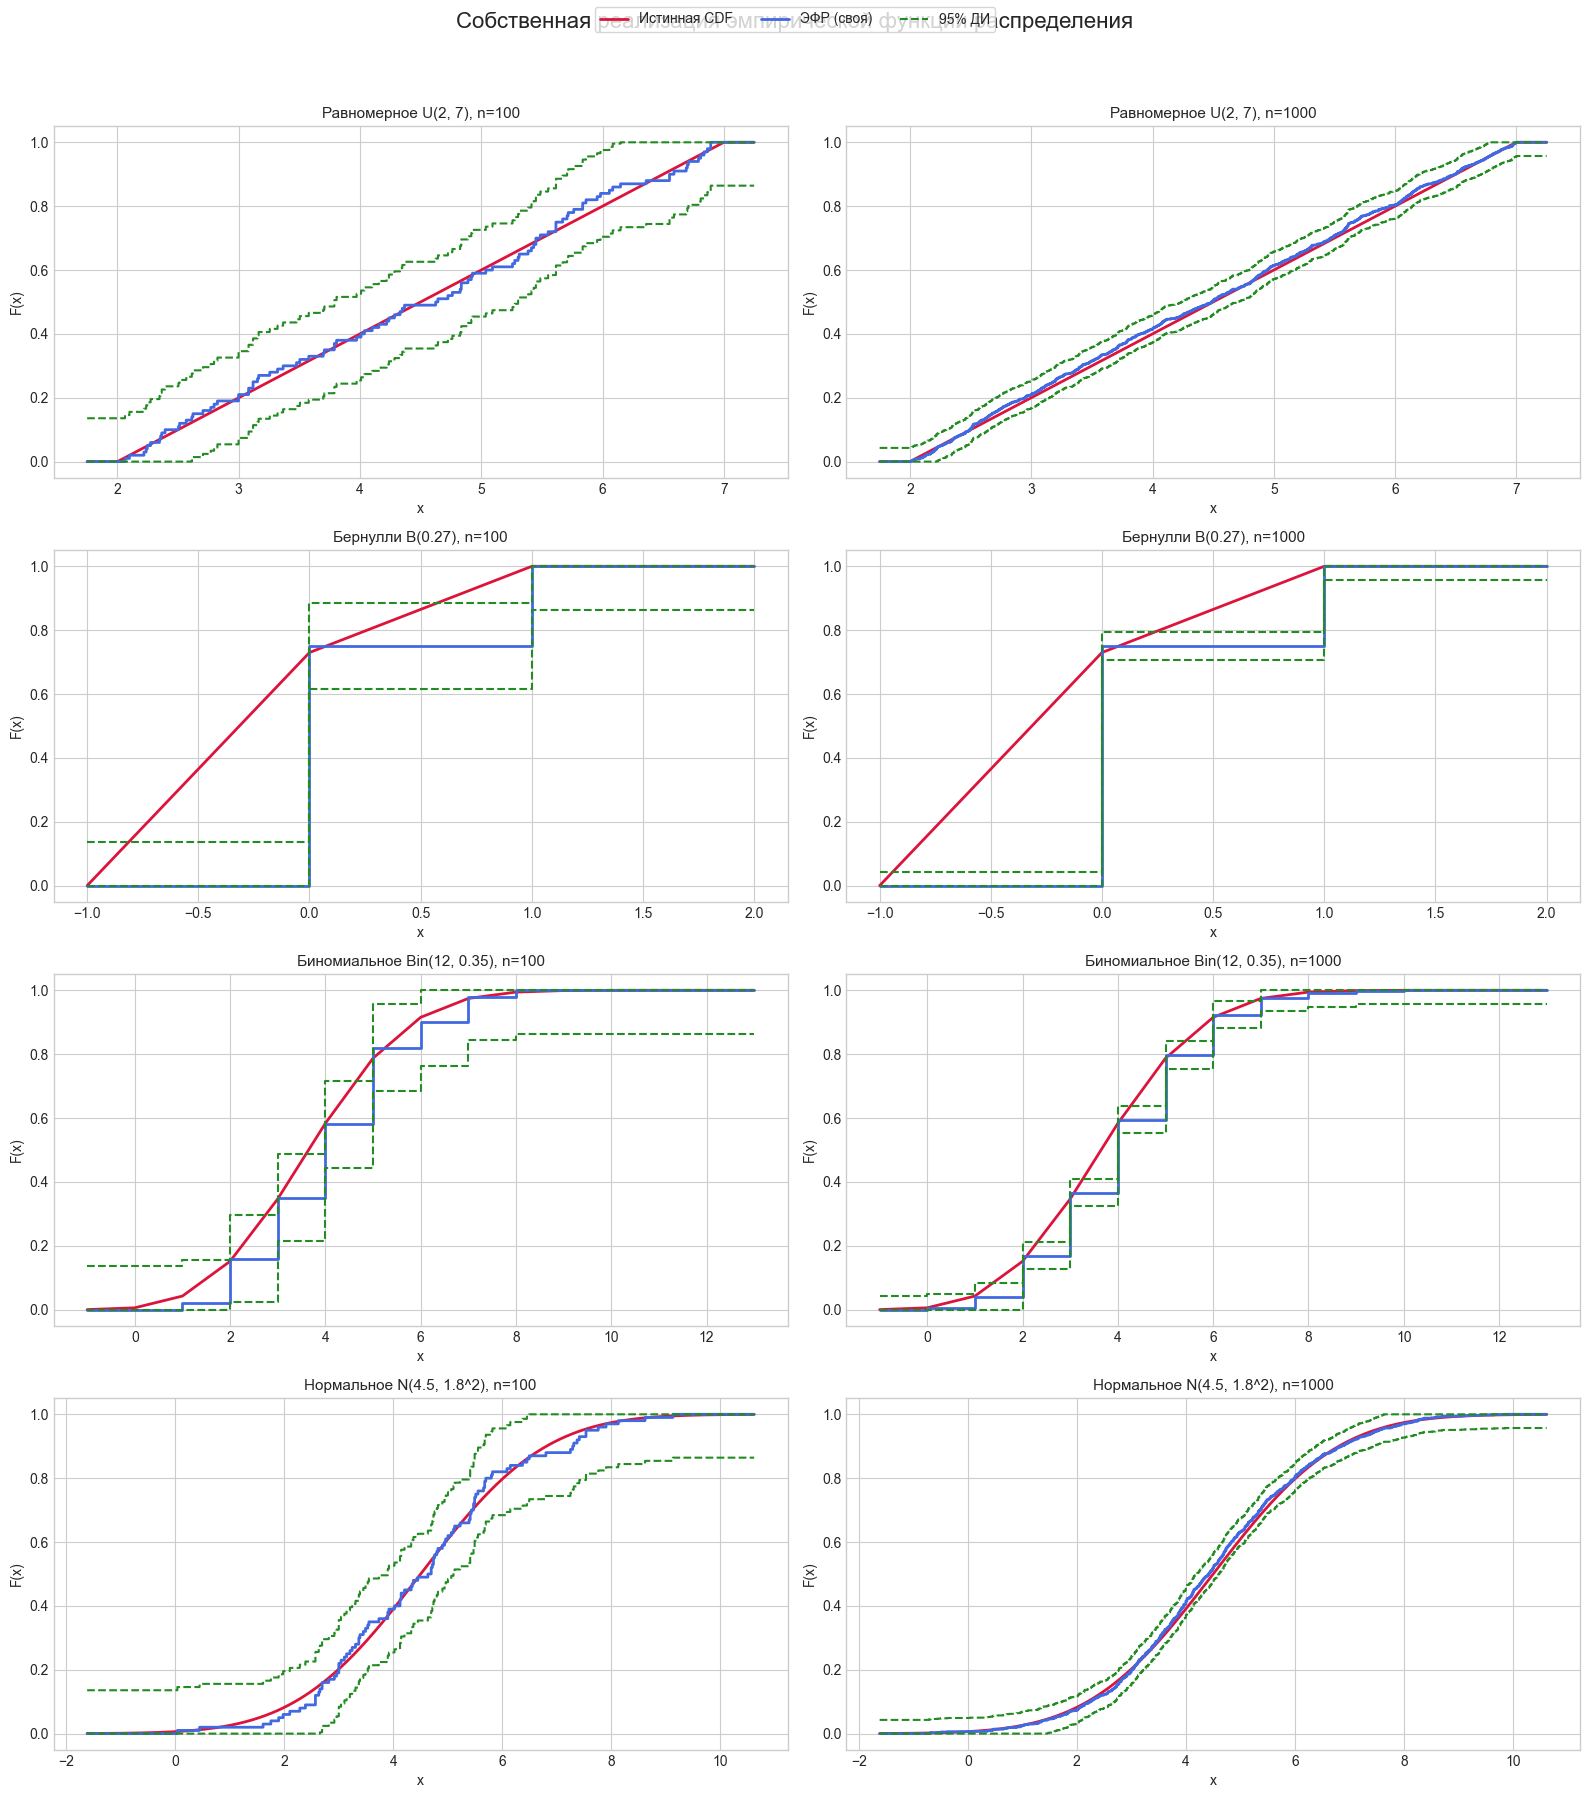
\includegraphics[width=\linewidth]{figures/custom_ecdf.png}
    \caption{Собственная реализация ЭФР и 95\%-го доверительного интервала}
\end{figure}

На следующем рисунке приведены результаты, полученные с помощью \texttt{scipy.stats.ecdf}. Значения ЭФР совпадают с собственной реализацией, а доверительные интервалы могут немного отличаться, так как в \texttt{SciPy} используется другой способ их построения.

\begin{figure}[H]
    \centering
    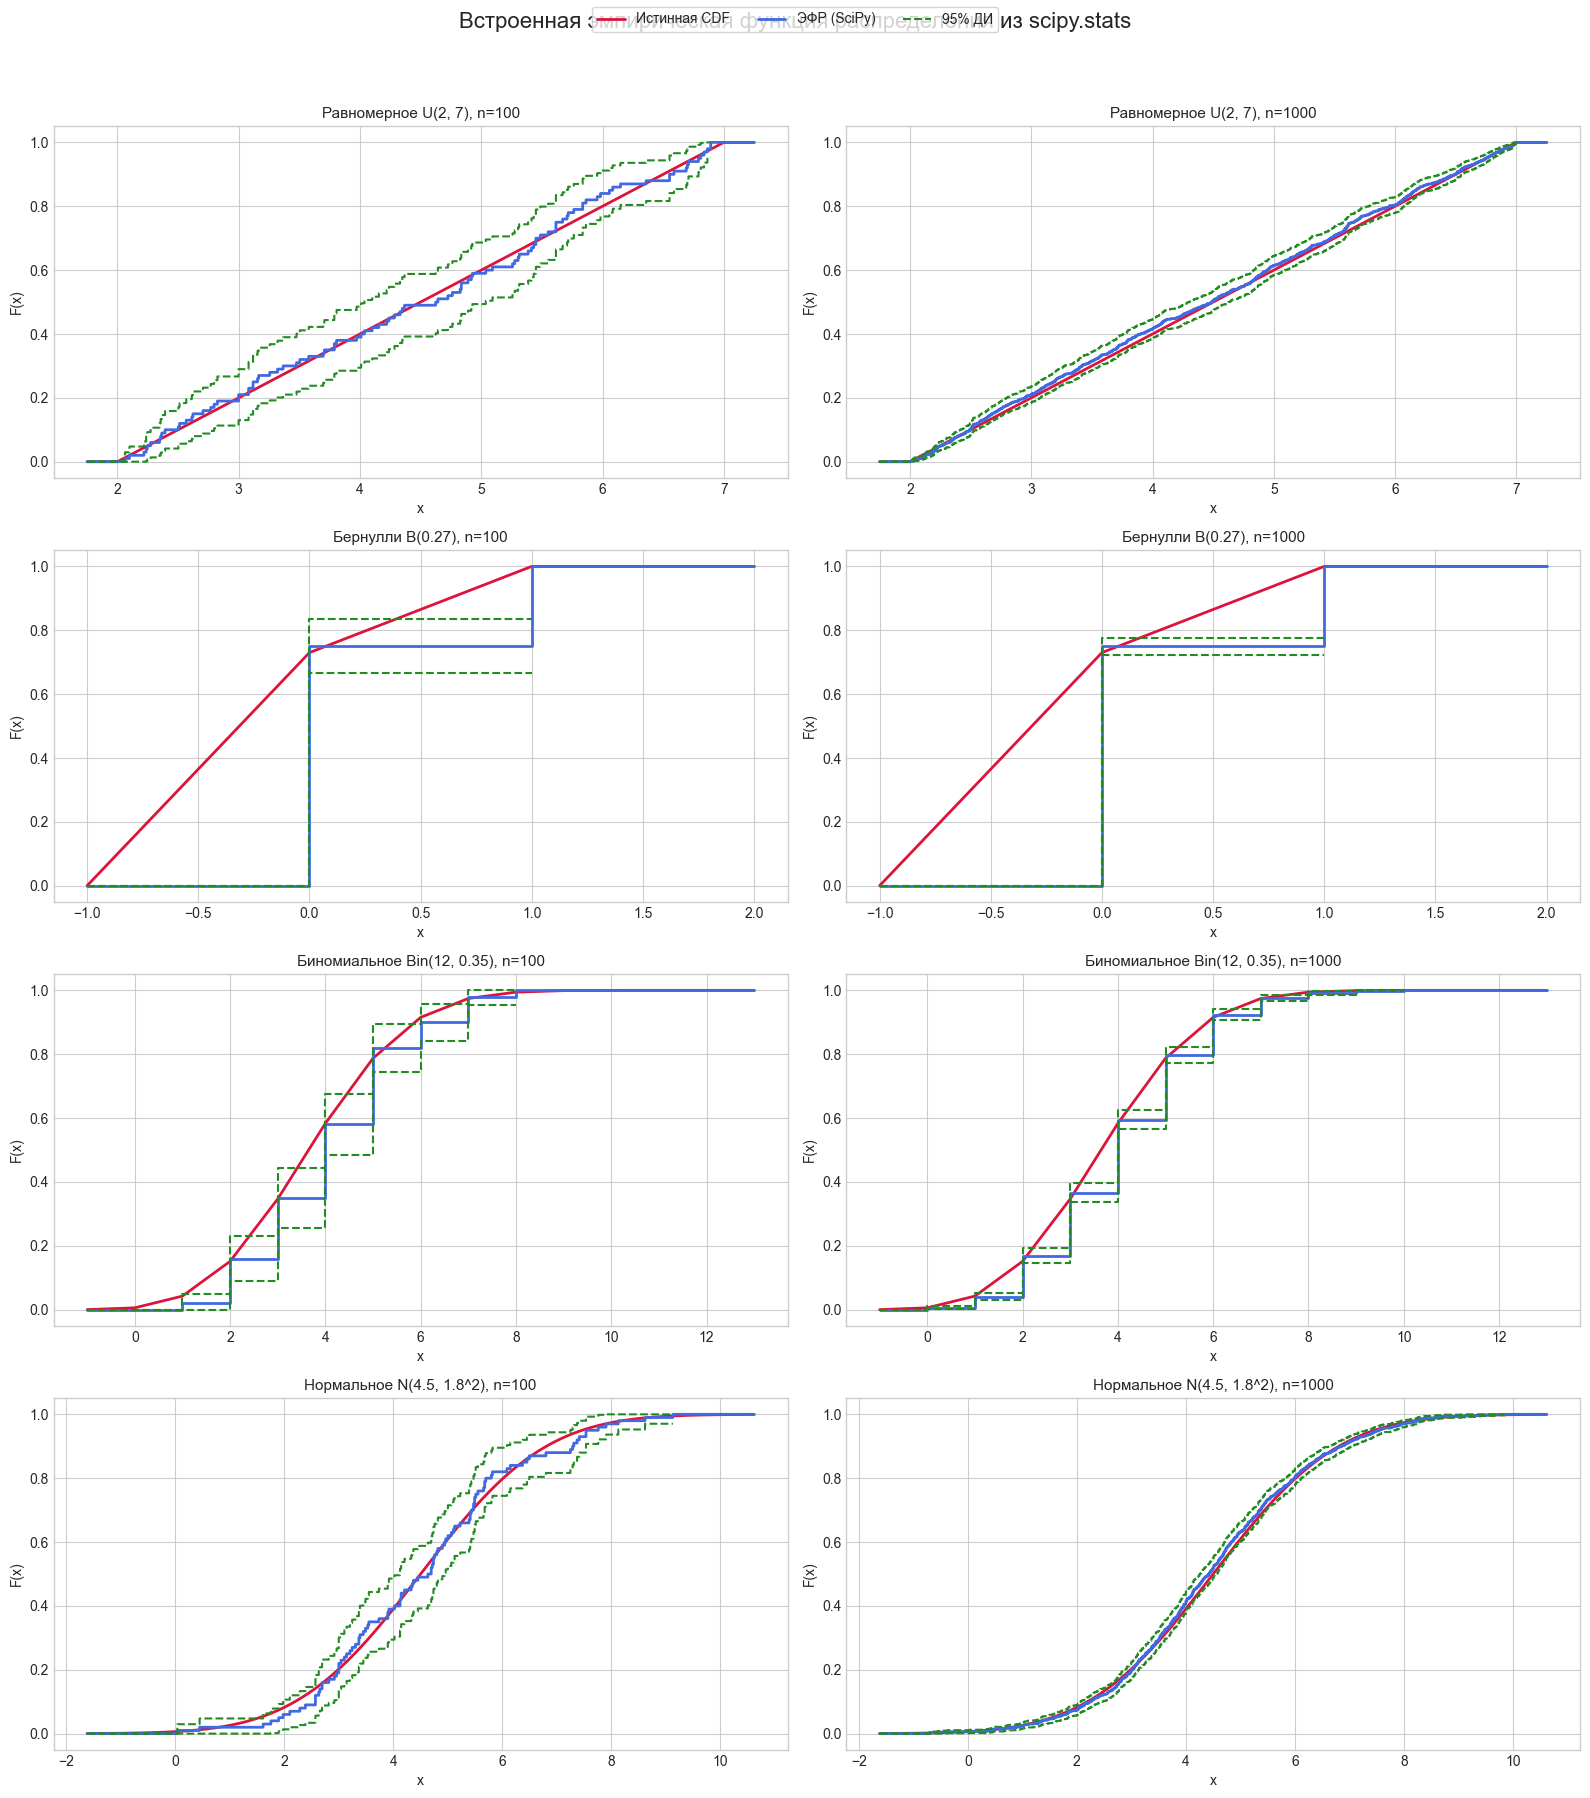
\includegraphics[width=\linewidth]{figures/scipy_ecdf.png}
    \caption{ЭФР и 95\%-й доверительный интервал с использованием \texttt{scipy.stats.ecdf}}
\end{figure}

\subsection{ Вывод }

В лабораторной работе была реализована собственная функция вычисления эмпирической функции распределения и 95\%-го доверительного интервала. Для всех восьми выборок построены графики истинной функции распределения, собственной ЭФР и встроенной ЭФР из \texttt{SciPy}.

С увеличением объёма выборки от \(100\) до \(1000\) эмпирическая функция распределения становится ближе к теоретической функции распределения, а доверительный интервал сужается. Это подтверждает корректность реализации и ожидаемое улучшение качества оценки при росте числа наблюдений.

\section{Полный код программы}

\lstinputlisting[caption={Код программы для лабораторной работы №3}]{lab3_code.py}

\end{document}
